\chapter{Requirement Specifications} \label{chap:reqs} \label{chap:requirements}

\section{Existing System}
Existing recruitment mechanisms and job aggregator platforms in the local and global context focus primarily on passive job posting and uncoordinated resume aggregation. Job postings are often published with minimal structural criteria, resumes are submitted as static documents into crowded email inboxes or unparsed databases, and candidate evaluation is handled manually or through primitive keyword-matching scripts \cite{parasuraman2021ats}. In conventional workflows, recruiters spend an average of only six seconds manually scanning each resume, leading to subjective evaluation biases, human cognitive fatigue, and high turnaround times. When first-generation legacy Applicant Tracking Systems (ATS) are deployed, they rely on rigid substring matching that rejects qualified applicants who omit exact keyword synonyms, while rewarding candidates who artificially ``stuff'' keywords into their CVs \cite{roy2020resume}. Furthermore, applicants face a total ``black hole'', receiving no diagnostic feedback regarding why their application was disqualified or what skills were missing.

Key limitations of existing systems include:
\begin{itemize}
    \item \textbf{Cognitive Fatigue and High Time-to-Hire:} Manual screening of hundreds of unstructured resumes causes severe operational bottlenecks and inconsistent candidate assessments.
    \item \textbf{Syntactic Rigidity and False Disqualifications:} Legacy keyword filters fail to recognize contextual synonyms, domain hierarchies, or transferrable technical competencies.
    \item \textbf{Vulnerability to Keyword Stuffing:} Naive keyword frequency parsers are easily manipulated by unqualified candidates who pack job description text into their resumes.
    \item \textbf{Complete Candidate Feedback Void:} Job seekers receive no transparency into their computed ATS compatibility scores or missing skill gaps.
    \item \textbf{Unverified Employer Postings:} Open job boards allow unverified accounts to post fraudulent listings, putting candidate personal data at risk.
    \item \textbf{Disjointed Pipeline Tracking:} Employers rely on separate offline spreadsheets to track candidate hiring stages due to lack of integrated stage management.
\end{itemize}

\section{Proposed System}
\textbf{RecruitSense} is proposed as an intelligent, multi-channel recruitment ecosystem, Applicant Tracking System (ATS), and Candidate Intelligence Platform engineered to streamline recruitment workflows, automate candidate screening, deliver explainable feedback, and provide recruiters with conversational resume deep-dives. The platform is architected as a decoupled, multi-tier microservices ecosystem consisting of:
\begin{enumerate}
    \item A responsive Single Page Application (SPA) frontend built with React 18, Vite, and Tailwind CSS.
    \item A cross-platform mobile application engineered with Flutter and Dart for Android and iOS.
    \item A high-throughput RESTful API gateway engineered with Laravel 11 and MySQL 8.0.
    \item An asynchronous AI inference microservice developed with Python FastAPI and Scikit-learn.
    \item A Retrieval-Augmented Generation (RAG) candidate intelligence engine powered by the ChromaDB vector database and sentence transformer embeddings (\texttt{all-MiniLM-L6-v2}) \cite{lewis2020rag, malkov2018hnsw}.
\end{enumerate}

Major capabilities of the proposed system include:
\begin{itemize}
    \item \textbf{Automated AI-Powered Resume Screening:} Converts unstructured PDF resumes into normalized text streams, extracts candidate competencies, and computes a multi-attribute ATS match score ($0\% - 100\%$) against job descriptions.
    \item \textbf{Candidate Retrieval-Augmented Generation (RAG) Chat:} Enables recruiters to ask natural-language questions about candidates, retrieving semantically relevant text chunks from resumes with source citation evidence.
    \item \textbf{Skill Gap Diagnostics and Automated Course Pathways:} Automatically categorizes competencies into matched, missing, and bonus skills, and provides rejected candidates with targeted online course recommendations to upskill.
    \item \textbf{Dynamic AI Assessment Quiz Generation:} Automatically generates technical multiple-choice quizzes tailored to required job skills for candidate pre-screening.
    \item \textbf{Multi-Channel Role-Based Workspaces:} Delivers synchronized, role-based dashboards on Web and Mobile for Job Seekers (profile, experience tracking, job alerts, recommended jobs, application tracking) and Corporate Recruiters (candidate discovery, Kanban pipeline, analytics, interview scheduling).
    \item \textbf{Live Community Feed and Professional Networking:} Provides interactive social networking feeds for job seekers and employers to share professional updates, insights, and industry discussions.
    \item \textbf{Corporate Email Domain Verification:} Protects job seekers by enforcing custom domain validation rules (\texttt{TrustedEmailDomain}) to prevent fraudulent employer registrations.
    \item \textbf{Structured Hiring Pipeline Management:} Enables recruiters to manage candidate lifecycles across dynamic stages (\textit{Applied} $\rightarrow$ \textit{Screening} $\rightarrow$ \textit{Shortlisted} $\rightarrow$ \textit{Interview} $\rightarrow$ \textit{Offer/Rejected}).
\end{itemize}

\section{Requirement Specifications}

\subsection{Functional Requirements}
Functional requirements define the specific behaviors, operations, and services that RecruitSense must provide to its users. They are derived directly from system use cases and stakeholder goals. Table \ref{tab:functional_reqs} enumerates all functional requirements with their unique identifiers and descriptions.

\begin{table}[h!]
\centering
\small
\caption{Functional Requirements for RecruitSense}
\label{tab:functional_reqs}
\begin{tabular}{|l|p{12cm}|}
\hline
\textbf{ID} & \textbf{Functional Requirement Description} \\ \hline
\textbf{FR-01} & \textbf{User Registration and Authentication:} Allow users to register as Job Seekers, Recruiters, or Admins and authenticate securely via Laravel Sanctum bearer tokens and Google OAuth. \\ \hline
\textbf{FR-02} & \textbf{Profile and Experience Management:} Enable Job Seekers and Employers to maintain profiles, experience records, bios, and account settings. \\ \hline
\textbf{FR-03} & \textbf{Corporate Domain Verification:} Validate recruiter registration emails against corporate domain whitelists, blocking public disposable email providers. \\ \hline
\textbf{FR-04} & \textbf{Create and Publish Job Vacancies:} Allow recruiters to create job postings with structured criteria (title, department, salary, description, required skills, experience). \\ \hline
\textbf{FR-05} & \textbf{Search and Multi-Filter Job Listings:} Provide job seekers with real-time job searching and multi-parameter filtering (keywords, location, employment type, salary). \\ \hline
\textbf{FR-06} & \textbf{Submit Job Application:} Enable job seekers to apply to vacancies by uploading their resume in PDF format with optional cover notes. \\ \hline
\textbf{FR-07} & \textbf{AI PDF Text Extraction:} Ingest uploaded resume documents and extract sanitized UTF-8 text streams page-by-page using the FastAPI AI microservice. \\ \hline
\textbf{FR-08} & \textbf{Skill Extraction and Boundary Matching:} Extract candidate skills using boundary-delimited regular expressions against a curated multi-domain technology taxonomy. \\ \hline
\textbf{FR-09} & \textbf{TF-IDF Cosine Similarity Computation:} Calculate contextual similarity between normalized resume text vectors and job description text vectors. \\ \hline
\textbf{FR-10} & \textbf{Composite ATS Score Formulation:} Compute a weighted ATS match percentage ($0\% - 100\%$) combining skill gap fulfillment and contextual TF-IDF similarity. \\ \hline
\textbf{FR-11} & \textbf{Skill Gap Diagnostics Visualization:} Display color-coded badges for matched skills, missing skills, and bonus skills to candidates and recruiters. \\ \hline
\textbf{FR-12} & \textbf{AI-Ranked Applicant Shortlist:} Display candidate applications to recruiters sorted in descending order of calculated ATS score. \\ \hline
\textbf{FR-13} & \textbf{Hiring Pipeline Stage Management:} Allow recruiters to transition candidate statuses across stages (\textit{Applied}, \textit{Screening}, \textit{Shortlisted}, \textit{Interview}, \textit{Offer}, \textit{Rejected}). \\ \hline
\textbf{FR-14} & \textbf{Interview Scheduling:} Enable recruiters to configure interview dates, times, and physical or virtual meeting locations for shortlisted candidates. \\ \hline
\textbf{FR-15} & \textbf{Save and Bookmark Jobs:} Allow job seekers to bookmark jobs of interest into a personal saved jobs list for future review. \\ \hline
\textbf{FR-16} & \textbf{Real-Time In-App Messaging:} Enable direct messaging between job seekers and recruiters to coordinate application details. \\ \hline
\textbf{FR-17} & \textbf{Notification System:} Dispatch real-time in-app alerts for application status changes, new messages, and scheduled interviews. \\ \hline
\textbf{FR-18} & \textbf{Report Fraudulent Postings:} Allow job seekers to report suspicious or misleading job listings for administrative investigation. \\ \hline
\textbf{FR-19} & \textbf{Admin Moderation Console:} Provide administrators with tools to moderate employers, review flagged listings, and suspend abusive user accounts. \\ \hline
\textbf{FR-20} & \textbf{Platform Analytics Dashboard:} Provide administrators and recruiters with statistical dashboards showing applicant distributions and match metrics. \\ \hline
\textbf{FR-21} & \textbf{Candidate RAG Conversational Chat:} Enable recruiters to query candidate qualifications through semantic dense vector search and grounded context generation using ChromaDB. \\ \hline
\textbf{FR-22} & \textbf{Cross-Platform Flutter Mobile Workspaces:} Deliver synchronized native mobile applications for Android and iOS providing candidate discovery, job alerts, and pipeline tracking. \\ \hline
\textbf{FR-23} & \textbf{Automated Skill Gap Course Recommendations:} Recommend curated online courses (Coursera, edX, Udemy) tailored to candidate missing competencies. \\ \hline
\textbf{FR-24} & \textbf{Automated AI Assessment Quiz Generation:} Dynamically generate multiple-choice skill assessment tests based on required vacancy competencies. \\ \hline
\textbf{FR-25} & \textbf{Community Feed and Professional Networking:} Provide a community discussion wall where users share professional posts, comments, and connection networks. \\ \hline
\end{tabular}
\end{table}

\subsection{Non-Functional Requirements}
Non-functional requirements specify quality constraints, security parameters, and operational attributes governing the system architecture. Table \ref{tab:non_functional_reqs} summarizes the key non-functional requirements.

\begin{table}[h!]
\centering
\small
\caption{Non-Functional Requirements for RecruitSense}
\label{tab:non_functional_reqs}
\begin{tabular}{|l|p{12cm}|}
\hline
\textbf{ID} & \textbf{Non-Functional Requirement Description} \\ \hline
\textbf{NFR-01} & \textbf{Performance and Latency:} Ensure standard REST API responses occur within $300\text{ ms}$, RAG semantic queries respond in under $1.5\text{ seconds}$, and ATS scoring executes under $2.0\text{ seconds}$. \\ \hline
\textbf{NFR-02} & \textbf{Authentication and Token Security:} Protect all authenticated API endpoints with Laravel Sanctum bearer tokens hashed with SHA-256 in database storage. \\ \hline
\textbf{NFR-03} & \textbf{Data Protection and Hashing:} Hash all user passwords using Bcrypt with a minimum work factor of 12 rounds to protect against brute-force attacks. \\ \hline
\textbf{NFR-04} & \textbf{Input Sanitization and SQLi Prevention:} Neutralize SQL injection vulnerabilities by executing all queries through Eloquent ORM parameterized statements. \\ \hline
\textbf{NFR-05} & \textbf{Multi-Platform Responsiveness and UI Fluidity:} Provide an intuitive web interface with Tailwind CSS and a mobile application running at consistent 60 frames-per-second. \\ \hline
\textbf{NFR-06} & \textbf{System Reliability and Fault Tolerance:} Gracefully handle AI microservice timeouts and document extraction errors without corrupting core database state. \\ \hline
\textbf{NFR-07} & \textbf{Horizontal Scalability and Async I/O:} Implement asynchronous non-blocking request processing via FastAPI and ChromaDB vector indexing. \\ \hline
\textbf{NFR-08} & \textbf{Secure File Storage:} Validate uploaded file MIME types, enforce a 5MB size limit, and obfuscate file names with randomized UUID hashes outside public web roots. \\ \hline
\textbf{NFR-09} & \textbf{Maintainability and Modular Architecture:} Adhere to standard MVC in Laravel, Provider pattern in Flutter, and service-oriented design in FastAPI. \\ \hline
\textbf{NFR-10} & \textbf{CORS and Transport Encryption:} Enforce HTTPS across all network channels and configure strict Cross-Origin Resource Sharing (CORS) whitelists. \\ \hline
\end{tabular}
\end{table}

\section{System Use Case Modeling}
Use case modeling provides a high-level visual representation of how system actors interact with RecruitSense. The system identifies four primary actors:
\begin{enumerate}
    \item \textbf{Guest / Unregistered Visitor:} Can browse public job listings and initiate registration.
    \item \textbf{Job Seeker (Candidate):} Can manage profiles, search and filter jobs, submit resumes, view ATS match scores and skill gap feedback, track application pipelines, and message recruiters.
    \item \textbf{Corporate Recruiter / Employer:} Can create company profiles, publish job postings with skill requirements, review AI-ranked candidate shortlists, update hiring pipeline stages, schedule interviews, and message candidates.
    \item \textbf{System Administrator:} Can oversee user management, verify corporate domains, moderate flagged content, and inspect platform analytics.
    \item \textbf{AI Screening Engine (System Actor):} Autonomously parses uploaded PDF documents, computes TF-IDF similarity vectors, and calculates ATS match scores.
\end{enumerate}

Figure \ref{fig:overall_usecase} illustrates the comprehensive system use case model for RecruitSense.

\begin{figure}[h!]
\centering
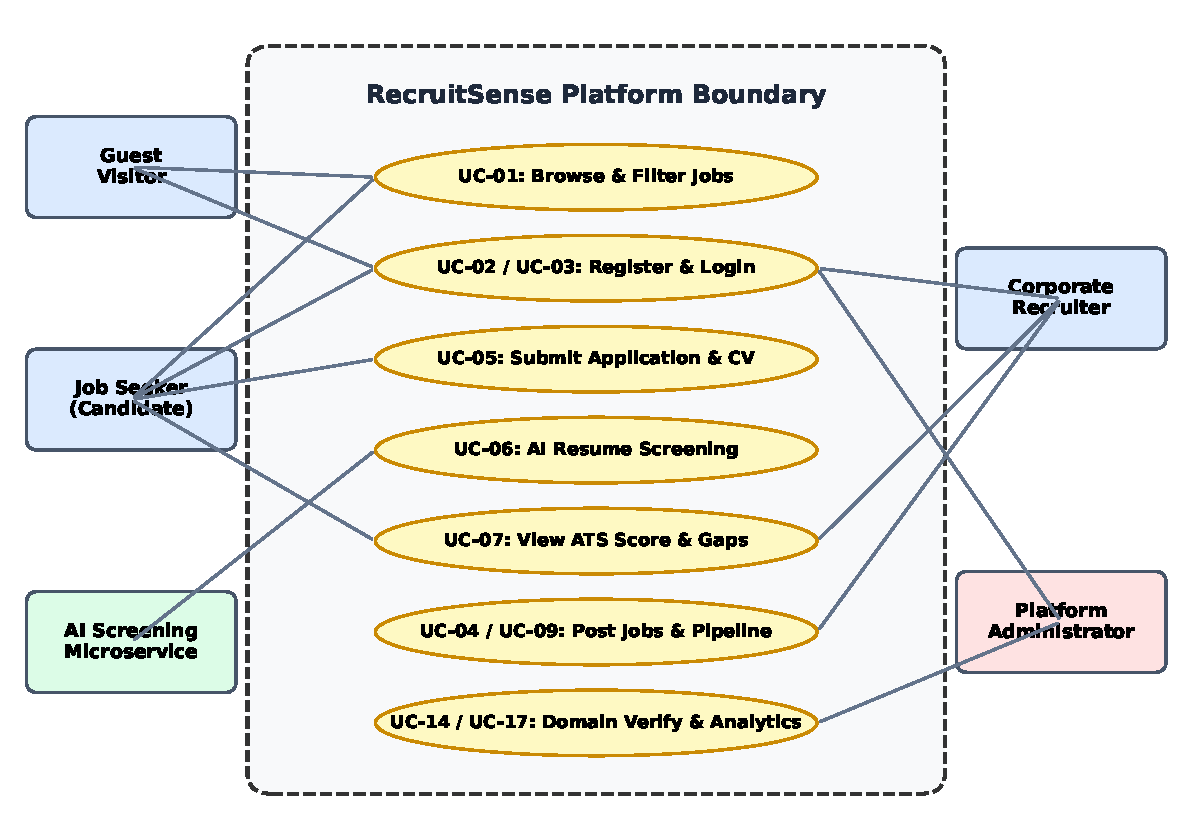
\includegraphics[width=0.85\linewidth]{figures/usecase_model.pdf}
\caption{System Use Case Model for RecruitSense}
\label{fig:overall_usecase}
\end{figure}

\section{Detailed Use Cases}

\subsection{Browse and Filter Jobs (UC-01)}
When a user accesses the RecruitSense web portal, they can immediately explore active job listings posted by verified employers. The browsing interface provides an intuitive search bar allowing users to enter job titles, technologies, or keywords. Users can refine search results using dynamic filters such as employment type (Full-time, Part-time, Remote, Contract), minimum salary range, and department category. Each listing card displays essential metadata, including job title, company name, location, salary badge, and required skills. Clicking a listing opens a comprehensive view detailing full responsibilities, candidate requirements, and an instant application trigger. Guests can freely browse all listings, while bookmarking jobs and submitting applications require an authenticated Job Seeker account. This workflow is modeled in Figure \ref{fig:uc01_diag} and specified in Table \ref{tab:uc01_spec}.

\begin{figure}[h!]
\centering
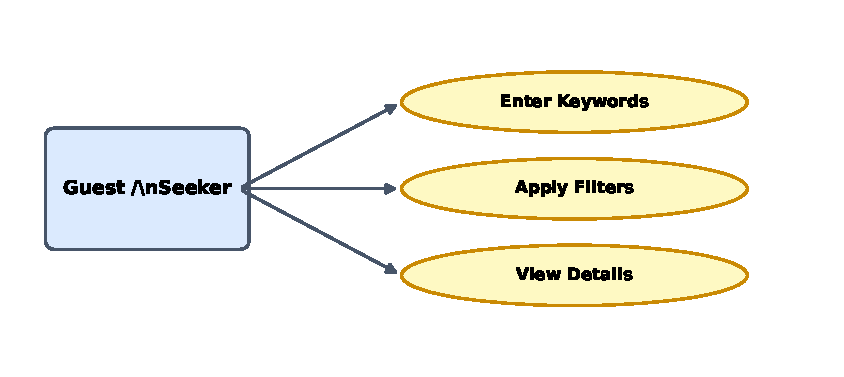
\includegraphics[width=0.65\linewidth]{figures/usecase_browse.pdf}
\caption{Browse and Filter Jobs Use Case Diagram (UC-01)}
\label{fig:uc01_diag}
\end{figure}

\begin{table}[h!]
\centering
\small
\caption{Use Case: Browse and Filter Jobs (UC-01)}
\label{tab:uc01_spec}
\begin{tabular}{|p{3.5cm}|p{11.5cm}|}
\hline
\textbf{Use Case ID} & UC-01 \\ \hline
\textbf{Use Case Name} & Browse and Filter Jobs \\ \hline
\textbf{Created By} & RecruitSense Engineering Team \\ \hline
\textbf{Last Updated By} & Lead System Architect \\ \hline
\textbf{Actors} & Guest, Registered Job Seeker \\ \hline
\textbf{Description} & User searches, filters, and views published job openings on the web portal. \\ \hline
\textbf{Trigger} & User accesses the platform job portal page. \\ \hline
\textbf{Preconditions} & Platform web service and database are operational; at least one active job exists. \\ \hline
\textbf{Postconditions} & Matching job vacancy cards and detailed modals are displayed to the user. \\ \hline
\textbf{Normal Flow} & 
\textbf{Actor Actions:} \newline
1. User enters keywords or selects job category. \newline
3. User selects filter criteria (Remote, Full-time, Salary). \newline
5. User clicks on a job card. \newline
\textbf{System Responses:} \newline
2. System queries database and retrieves matching active listings. \newline
4. System dynamically updates the list view without full page reload. \newline
6. System displays full job description modal with required skills. \\ \hline
\textbf{Alternative Flows} & 1. Job Seeker saves job to bookmarks. \newline 2. User clears all filters to view full catalogue. \\ \hline
\textbf{Exceptions} & 1. No jobs match search criteria (System renders friendly empty-state). \newline 2. Network connectivity failure. \\ \hline
\end{tabular}
\end{table}

\subsection{Register User with Role Assignment (UC-02)}
When a new user visits RecruitSense, they can register an account by providing their full name, email address, password, and selecting their intended operational role: \textit{Job Seeker} or \textit{Corporate Recruiter / Employer}. The system validates that the email address is well-formed and unique. For corporate recruiter accounts, the custom validation rule (\texttt{TrustedEmailDomain}) verifies that the email domain is an authentic business domain rather than a personal or disposable provider. Once validated, the backend hashes the password using Bcrypt, creates the database record, issues a Laravel Sanctum Personal Access Token, and redirects the user to their role-specific onboarding dashboard. This workflow is shown in Figure \ref{fig:uc02_diag} and detailed in Table \ref{tab:uc02_spec}.

\begin{figure}[h!]
\centering
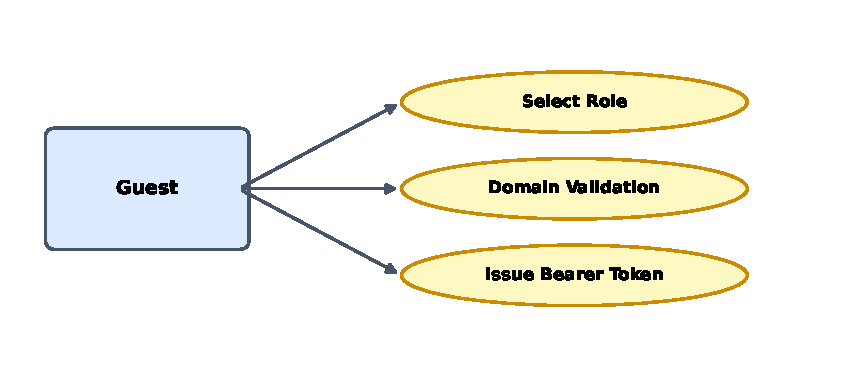
\includegraphics[width=0.65\linewidth]{figures/usecase_register.pdf}
\caption{Register User Use Case Diagram (UC-02)}
\label{fig:uc02_diag}
\end{figure}

\begin{table}[h!]
\centering
\small
\caption{Use Case: Register User with Role Assignment (UC-02)}
\label{tab:uc02_spec}
\begin{tabular}{|p{3.5cm}|p{11.5cm}|}
\hline
\textbf{Use Case ID} & UC-02 \\ \hline
\textbf{Use Case Name} & Register User with Role Assignment \\ \hline
\textbf{Created By} & RecruitSense Engineering Team \\ \hline
\textbf{Last Updated By} & Lead System Architect \\ \hline
\textbf{Actors} & Guest (New User) \\ \hline
\textbf{Description} & New user creates an account with role-specific validation and domain verification. \\ \hline
\textbf{Trigger} & User clicks ``Sign Up'' on the web navigation bar. \\ \hline
\textbf{Preconditions} & User possesses a valid, unique email address. \\ \hline
\textbf{Postconditions} & User account is created; Sanctum Bearer token is issued and stored in client state. \\ \hline
\textbf{Normal Flow} & 
\textbf{Actor Actions:} \newline
1. User enters name, email, password, and selects role (\textit{Job Seeker} / \textit{Employer}). \newline
3. User submits registration form. \newline
\textbf{System Responses:} \newline
2. System validates input formats, password length ($\ge 8$), and domain legitimacy. \newline
4. System hashes password via Bcrypt, inserts record, generates token, and redirects to dashboard. \\ \hline
\textbf{Alternative Flows} & 1. User registers with Google Single Sign-On (OAuth2). \\ \hline
\textbf{Exceptions} & 1. Email already registered (HTTP 422 error returned). \newline 2. Employer email uses blacklisted disposable domain. \\ \hline
\end{tabular}
\end{table}

\subsection{User Login and Token Authentication (UC-03)}
When a registered user accesses RecruitSense, they authenticate by entering their registered email and password. The Laravel backend verifies credential validity against the database, checks whether the account is active or suspended, generates a cryptographically secure Sanctum personal access token, and returns the token along with user profile metadata. The React client persists the token securely and mounts the appropriate dashboard based on user role. This workflow is shown in Figure \ref{fig:uc03_diag} and described in Table \ref{tab:uc03_spec}.

\begin{figure}[h!]
\centering
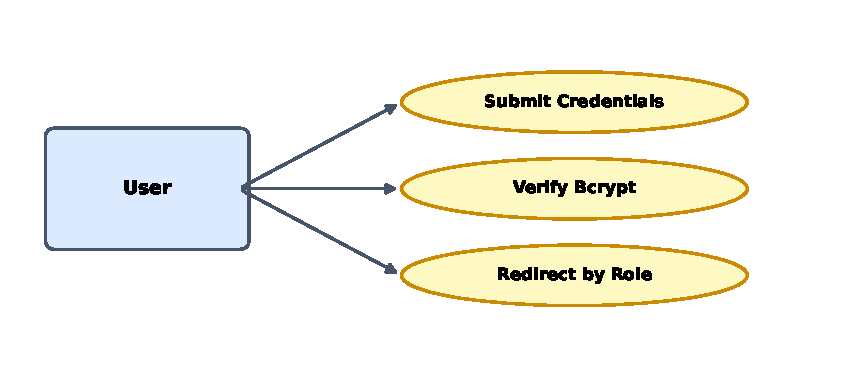
\includegraphics[width=0.65\linewidth]{figures/usecase_login.pdf}
\caption{User Login Use Case Diagram (UC-03)}
\label{fig:uc03_diag}
\end{figure}

\begin{table}[h!]
\centering
\small
\caption{Use Case: User Login and Token Authentication (UC-03)}
\label{tab:uc03_spec}
\begin{tabular}{|p{3.5cm}|p{11.5cm}|}
\hline
\textbf{Use Case ID} & UC-03 \\ \hline
\textbf{Use Case Name} & User Login and Token Authentication \\ \hline
\textbf{Created By} & RecruitSense Engineering Team \\ \hline
\textbf{Last Updated By} & Lead System Architect \\ \hline
\textbf{Actors} & Registered User (Job Seeker, Recruiter, Admin) \\ \hline
\textbf{Description} & Authenticate user credentials and establish a secure, tokenized session. \\ \hline
\textbf{Trigger} & User clicks ``Login'' and submits credentials. \\ \hline
\textbf{Preconditions} & User account exists and is not suspended. \\ \hline
\textbf{Postconditions} & Bearer token generated and user authenticated into role-specific dashboard. \\ \hline
\textbf{Normal Flow} & 
\textbf{Actor Actions:} \newline
1. User enters email and password. \newline
3. User clicks ``Login''. \newline
\textbf{System Responses:} \newline
2. System validates input syntax. \newline
4. System verifies Bcrypt hash, checks account status, issues Sanctum token, and redirects by role. \\ \hline
\textbf{Alternative Flows} & 1. User resets forgotten password via email reset token. \\ \hline
\textbf{Exceptions} & 1. Invalid credentials entered (HTTP 401 Unauthorized). \newline 2. Account is suspended (HTTP 403 Forbidden). \\ \hline
\end{tabular}
\end{table}

\subsection{Create and Publish Job Vacancy (UC-04)}
Corporate recruiters can create and publish new job vacancies through a dedicated posting interface. The recruiter provides the Job Title, Department, Location, Employment Type, Compensation Range, detailed Job Description, Minimum Experience Years, and explicit Required Technical Skills. The system validates the inputs, ensures the employer's company profile is verified, persists the vacancy to MySQL, and immediately publishes the listing to the public job board. This workflow is shown in Figure \ref{fig:uc04_diag} and summarized in Table \ref{tab:uc04_spec}.

\begin{figure}[h!]
\centering
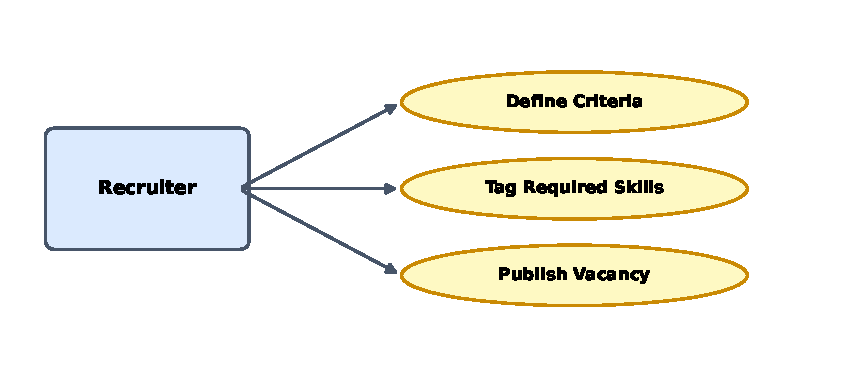
\includegraphics[width=0.65\linewidth]{figures/usecase_post_job.pdf}
\caption{Create and Publish Job Vacancy Use Case Diagram (UC-04)}
\label{fig:uc04_diag}
\end{figure}

\begin{table}[h!]
\centering
\small
\caption{Use Case: Create and Publish Job Vacancy (UC-04)}
\label{tab:uc04_spec}
\begin{tabular}{|p{3.5cm}|p{11.5cm}|}
\hline
\textbf{Use Case ID} & UC-04 \\ \hline
\textbf{Use Case Name} & Create and Publish Job Vacancy \\ \hline
\textbf{Created By} & RecruitSense Engineering Team \\ \hline
\textbf{Last Updated By} & Lead System Architect \\ \hline
\textbf{Actors} & Corporate Recruiter / Employer \\ \hline
\textbf{Description} & Recruiter defines job details, tags required skills, and publishes an active opening. \\ \hline
\textbf{Trigger} & Recruiter clicks ``Post a New Job'' on the recruiter dashboard. \\ \hline
\textbf{Preconditions} & Recruiter is authenticated and possesses a verified company profile. \\ \hline
\textbf{Postconditions} & A new job record is inserted into the \texttt{job\_postings} table with status \texttt{'active'}. \\ \hline
\textbf{Normal Flow} & 
\textbf{Actor Actions:} \newline
1. Recruiter fills out job posting form (title, department, salary, description). \newline
3. Recruiter tags required technical skills (e.g., React, Laravel, MySQL). \newline
5. Recruiter clicks ``Publish Job''. \newline
\textbf{System Responses:} \newline
2. System validates input constraints. \newline
4. System parses skill tokens. \newline
6. System persists record, activates listing, and confirms publication. \\ \hline
\textbf{Alternative Flows} & 1. Recruiter saves job as a \texttt{'draft'} for later editing. \\ \hline
\textbf{Exceptions} & 1. Required fields missing (System displays form validation errors). \\ \hline
\end{tabular}
\end{table}

\subsection{Submit Job Application with Resume Upload (UC-05)}
When a job seeker discovers a relevant job opening, they submit their application by uploading their resume in PDF format. The backend validates file format and size constraints ($\le 5\text{MB}$), encrypts and stores the file on secure disk storage, and automatically triggers the internal AI screening microservice to parse the document and calculate the candidate's ATS match score. This workflow is shown in Figure \ref{fig:uc05_diag} and specified in Table \ref{tab:uc05_spec}.

\begin{figure}[h!]
\centering
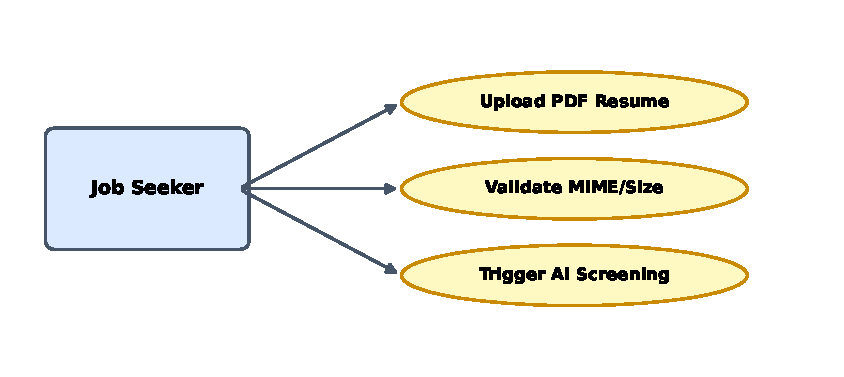
\includegraphics[width=0.65\linewidth]{figures/usecase_apply.pdf}
\caption{Submit Job Application Use Case Diagram (UC-05)}
\label{fig:uc05_diag}
\end{figure}

\begin{table}[h!]
\centering
\small
\caption{Use Case: Submit Job Application with Resume Upload (UC-05)}
\label{tab:uc05_spec}
\begin{tabular}{|p{3.5cm}|p{11.5cm}|}
\hline
\textbf{Use Case ID} & UC-05 \\ \hline
\textbf{Use Case Name} & Submit Job Application with Resume Upload \\ \hline
\textbf{Created By} & RecruitSense Engineering Team \\ \hline
\textbf{Last Updated By} & Lead System Architect \\ \hline
\textbf{Actors} & Job Seeker \\ \hline
\textbf{Description} & Candidate submits an application with PDF resume upload triggering automated screening. \\ \hline
\textbf{Trigger} & Candidate clicks ``Apply Now'' on a job details modal. \\ \hline
\textbf{Preconditions} & Candidate is authenticated; target job vacancy is active. \\ \hline
\textbf{Postconditions} & Application record created; resume stored; ATS score evaluated. \\ \hline
\textbf{Normal Flow} & 
\textbf{Actor Actions:} \newline
1. Candidate selects resume file (PDF) and enters optional cover note. \newline
3. Candidate clicks ``Submit Application''. \newline
\textbf{System Responses:} \newline
2. System verifies PDF MIME type and ensures size $\le 5\text{MB}$. \newline
4. System writes file to disk, dispatches payload to Flask AI service, persists calculated ATS score, and renders confirmation. \\ \hline
\textbf{Alternative Flows} & 1. Candidate uses previously uploaded profile resume. \\ \hline
\textbf{Exceptions} & 1. File exceeds 5MB or invalid extension (HTTP 422 error). \newline 2. Candidate has already applied to this posting (Duplicate prevention). \\ \hline
\end{tabular}
\end{table}

\subsection{Automated AI Resume Parsing and Semantic ATS Screening (UC-06)}
As an autonomous system actor, the Python Flask AI microservice receives the binary resume stream and job vacancy criteria from the Laravel backend. It extracts the raw text stream using PyPDF2, sanitizes punctuation and whitespace, executes boundary-delimited regex matching against required and bonus skill dictionaries, computes the TF-IDF vector matrix, and calculates the cosine similarity score. The structured evaluation is returned as JSON to the backend. This workflow is shown in Figure \ref{fig:uc06_diag} and detailed in Table \ref{tab:uc06_spec}.

\begin{figure}[h!]
\centering
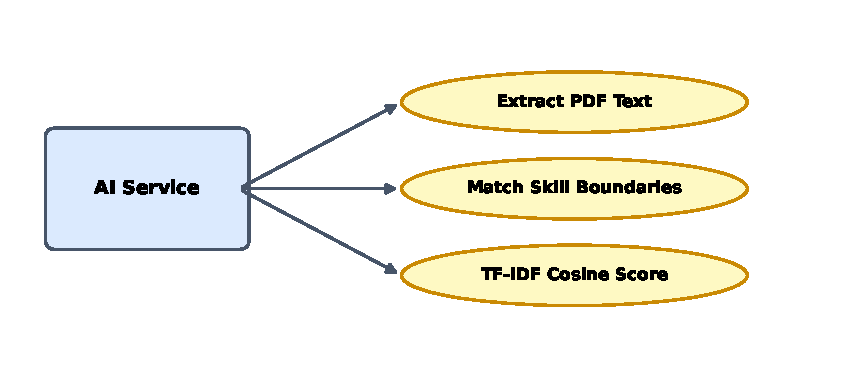
\includegraphics[width=0.65\linewidth]{figures/usecase_ai_screening.pdf}
\caption{AI Resume Screening Use Case Diagram (UC-06)}
\label{fig:uc06_diag}
\end{figure}

\begin{table}[h!]
\centering
\small
\caption{Use Case: AI Resume Parsing and ATS Screening (UC-06)}
\label{tab:uc06_spec}
\begin{tabular}{|p{3.5cm}|p{11.5cm}|}
\hline
\textbf{Use Case ID} & UC-06 \\ \hline
\textbf{Use Case Name} & Automated AI Resume Parsing and Semantic ATS Screening \\ \hline
\textbf{Created By} & RecruitSense Engineering Team \\ \hline
\textbf{Last Updated By} & Lead System Architect \\ \hline
\textbf{Actors} & AI Screening Microservice (System Actor) \\ \hline
\textbf{Description} & Autonomous microservice processes PDF text, extracts skills, and computes similarity scores. \\ \hline
\textbf{Trigger} & Laravel backend sends HTTP POST request to \texttt{/analyze-resume}. \\ \hline
\textbf{Preconditions} & Valid PDF stream and job description strings provided in payload. \\ \hline
\textbf{Postconditions} & Structured JSON evaluation returned containing scores, matched skills, and skill gaps. \\ \hline
\textbf{Normal Flow} & 
\textbf{System Actions (Backend $\rightarrow$ AI Service):} \newline
1. Backend sends multipart request with resume and required skills. \newline
2. AI Service extracts raw text from PDF via \texttt{pdf\_extractor}. \newline
3. AI Service matches required skills and identifies missing skill gaps. \newline
4. AI Service builds TF-IDF matrix and calculates cosine similarity percentage. \newline
5. AI Service returns HTTP 200 with structured JSON evaluation payload. \\ \hline
\textbf{Alternative Flows} & 1. AI service extracts bonus skills outside the required skills list. \\ \hline
\textbf{Exceptions} & 1. PDF has no extractable text layer (HTTP 422 error). \newline 2. Memory limit exceeded on oversized documents. \\ \hline
\end{tabular}
\end{table}

\subsection{View ATS Match Diagnostics and Skill Gap Analysis (UC-07)}
Job seekers and recruiters can view granular, transparent ATS evaluation breakdowns for any submitted application. The web interface displays the overall ATS Match Percentage, a visual gauge, a green badge list of verified matched skills, a red badge list of identified missing skills, and bonus competencies. This eliminates the ATS black box and provides candidates with clear career development feedback. This workflow is shown in Figure \ref{fig:uc07_diag} and specified in Table \ref{tab:uc07_spec}.

\begin{figure}[h!]
\centering
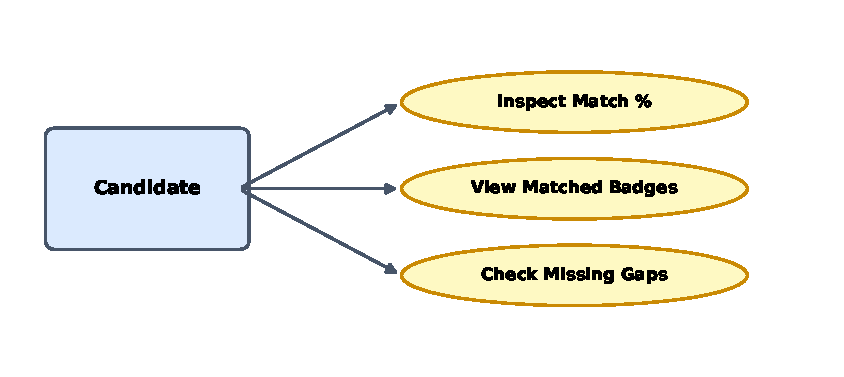
\includegraphics[width=0.65\linewidth]{figures/usecase_ats_score.pdf}
\caption{View ATS Score Diagnostics Use Case Diagram (UC-07)}
\label{fig:uc07_diag}
\end{figure}

\begin{table}[h!]
\centering
\small
\caption{Use Case: View ATS Match Diagnostics and Skill Gap Analysis (UC-07)}
\label{tab:uc07_spec}
\begin{tabular}{|p{3.5cm}|p{11.5cm}|}
\hline
\textbf{Use Case ID} & UC-07 \\ \hline
\textbf{Use Case Name} & View ATS Match Diagnostics and Skill Gap Analysis \\ \hline
\textbf{Created By} & RecruitSense Engineering Team \\ \hline
\textbf{Last Updated By} & Lead System Architect \\ \hline
\textbf{Actors} & Job Seeker, Corporate Recruiter \\ \hline
\textbf{Description} & Display comprehensive ATS score breakdown, matched skills, and missing skill badges. \\ \hline
\textbf{Trigger} & User clicks ``View ATS Breakdown'' on an application card. \\ \hline
\textbf{Preconditions} & Application exists and has been screened by the AI engine. \\ \hline
\textbf{Postconditions} & Diagnostic score modal is rendered with color-coded skill badges. \\ \hline
\textbf{Normal Flow} & 
\textbf{Actor Actions:} \newline
1. User navigates to application details. \newline
\textbf{System Responses:} \newline
2. System retrieves application record and associated \texttt{skill\_gaps} data. \newline
3. System renders overall match percentage, matched skills (green), and missing skills (red). \\ \hline
\textbf{Alternative Flows} & 1. Recruiter downloads extracted candidate summary report. \\ \hline
\textbf{Exceptions} & 1. Application is pending asynchronous screening calculation. \\ \hline
\end{tabular}
\end{table}

\subsection{Review AI-Ranked Candidate Shortlist (UC-08)}
Recruiters can inspect all applications received for a particular job vacancy, automatically sorted in descending order of calculated ATS Match Score. Recruiters can apply threshold filters (e.g., show only candidates with $\ge 80\%$ match), inspect extracted resume texts, compare applicant skill distributions, and identify top talent within seconds. This workflow is shown in Figure \ref{fig:uc08_diag} and detailed in Table \ref{tab:uc08_spec}.

\begin{figure}[h!]
\centering
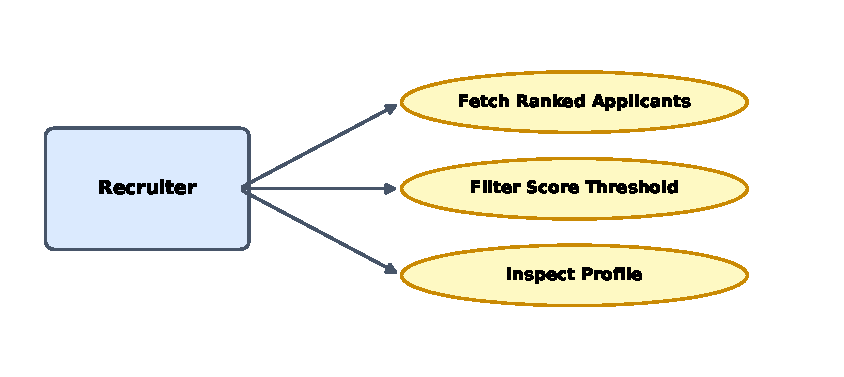
\includegraphics[width=0.65\linewidth]{figures/usecase_shortlist.pdf}
\caption{Review AI-Ranked Candidate Shortlist Use Case Diagram (UC-08)}
\label{fig:uc08_diag}
\end{figure}

\begin{table}[h!]
\centering
\small
\caption{Use Case: Review AI-Ranked Candidate Shortlist (UC-08)}
\label{tab:uc08_spec}
\begin{tabular}{|p{3.5cm}|p{11.5cm}|}
\hline
\textbf{Use Case ID} & UC-08 \\ \hline
\textbf{Use Case Name} & Review AI-Ranked Candidate Shortlist \\ \hline
\textbf{Created By} & RecruitSense Engineering Team \\ \hline
\textbf{Last Updated By} & Lead System Architect \\ \hline
\textbf{Actors} & Corporate Recruiter / Employer \\ \hline
\textbf{Description} & Recruiter reviews candidate applications sorted by AI match score with filter controls. \\ \hline
\textbf{Trigger} & Recruiter selects ``Manage Applicants'' for an active job posting. \\ \hline
\textbf{Preconditions} & Recruiter is authenticated; job posting has received at least one application. \\ \hline
\textbf{Postconditions} & Tabular candidate ranking list is displayed with score metrics. \\ \hline
\textbf{Normal Flow} & 
\textbf{Actor Actions:} \newline
1. Recruiter selects job posting. \newline
3. Recruiter adjusts minimum score slider (e.g., $75\%$). \newline
5. Recruiter clicks on top-ranked candidate profile. \newline
\textbf{System Responses:} \newline
2. System queries \texttt{applications} joined with \texttt{job\_seekers}, sorted by \texttt{ats\_score DESC}. \newline
4. System filters list dynamically. \newline
6. System displays detailed candidate profile and resume preview. \\ \hline
\textbf{Alternative Flows} & 1. Recruiter exports shortlisted candidate table to CSV. \\ \hline
\textbf{Exceptions} & 1. Job posting has received zero applicants (System displays empty state). \\ \hline
\end{tabular}
\end{table}

\subsection{Manage Hiring Pipeline Status (UC-09)}
Recruiters can transition candidate applications through the hiring stages (\textit{Applied} $\rightarrow$ \textit{Screening} $\rightarrow$ \textit{Shortlisted} $\rightarrow$ \textit{Interview Scheduled} $\rightarrow$ \textit{Offer Extended} $\rightarrow$ \textit{Accepted / Rejected}). Changing status immediately updates the candidate's tracking dashboard and triggers automated notification alerts. This workflow is shown in Figure \ref{fig:uc09_diag} and specified in Table \ref{tab:uc09_spec}.

\begin{figure}[h!]
\centering
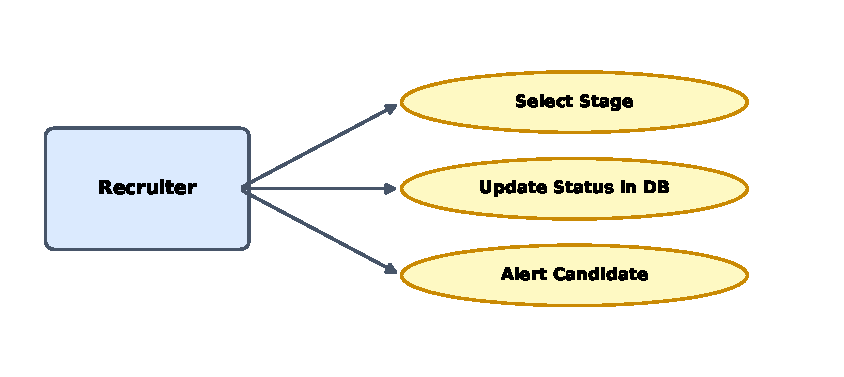
\includegraphics[width=0.65\linewidth]{figures/usecase_pipeline.pdf}
\caption{Manage Hiring Pipeline Status Use Case Diagram (UC-09)}
\label{fig:uc09_diag}
\end{figure}

\begin{table}[h!]
\centering
\small
\caption{Use Case: Manage Hiring Pipeline Status (UC-09)}
\label{tab:uc09_spec}
\begin{tabular}{|p{3.5cm}|p{11.5cm}|}
\hline
\textbf{Use Case ID} & UC-09 \\ \hline
\textbf{Use Case Name} & Manage Hiring Pipeline Status \\ \hline
\textbf{Created By} & RecruitSense Engineering Team \\ \hline
\textbf{Last Updated By} & Lead System Architect \\ \hline
\textbf{Actors} & Corporate Recruiter / Employer \\ \hline
\textbf{Description} & Recruiter advances candidate applications across hiring funnel stages. \\ \hline
\textbf{Trigger} & Recruiter changes the status dropdown on an applicant card. \\ \hline
\textbf{Preconditions} & Recruiter is authenticated and owns the job posting associated with the application. \\ \hline
\textbf{Postconditions} & Application status is updated in MySQL; notification event dispatched. \\ \hline
\textbf{Normal Flow} & 
\textbf{Actor Actions:} \newline
1. Recruiter selects new stage (e.g., \textit{Shortlisted} or \textit{Interview Scheduled}). \newline
3. Recruiter confirms stage update. \newline
\textbf{System Responses:} \newline
2. System validates transition validity. \newline
4. System updates \texttt{applications.status}, logs audit history, and sends candidate notification. \\ \hline
\textbf{Alternative Flows} & 1. Recruiter enters internal hiring remarks visible only to company staff. \\ \hline
\textbf{Exceptions} & 1. Candidate has withdrawn application (Status change blocked). \\ \hline
\end{tabular}
\end{table}

\subsection{Edit and Update Job Vacancy (UC-10)}
Recruiters can modify details of existing job postings (e.g., updating salary range, revising required skills, or extending application deadlines). The system loads current data, validates updates, persists changes, and logs modifications for auditing. This workflow is shown in Figure \ref{fig:uc10_diag} and detailed in Table \ref{tab:uc10_spec}.

\begin{figure}[h!]
\centering
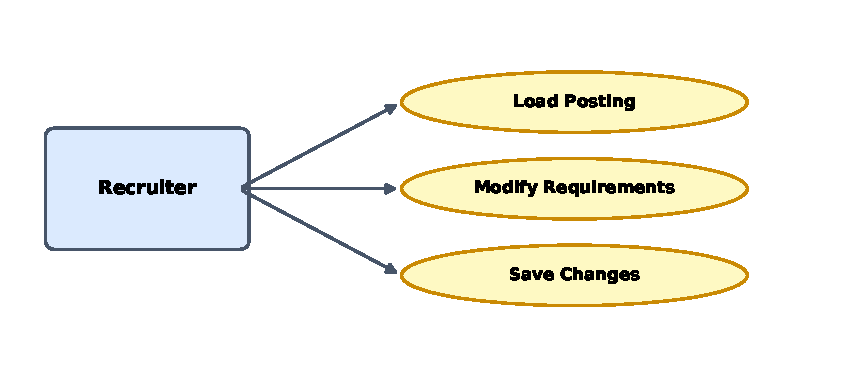
\includegraphics[width=0.65\linewidth]{figures/usecase_edit_job.pdf}
\caption{Edit Job Vacancy Use Case Diagram (UC-10)}
\label{fig:uc10_diag}
\end{figure}

\begin{table}[h!]
\centering
\small
\caption{Use Case: Edit and Update Job Vacancy (UC-10)}
\label{tab:uc10_spec}
\begin{tabular}{|p{3.5cm}|p{11.5cm}|}
\hline
\textbf{Use Case ID} & UC-10 \\ \hline
\textbf{Use Case Name} & Edit and Update Job Vacancy \\ \hline
\textbf{Created By} & RecruitSense Engineering Team \\ \hline
\textbf{Last Updated By} & Lead System Architect \\ \hline
\textbf{Actors} & Corporate Recruiter / Employer \\ \hline
\textbf{Description} & Recruiter modifies information, requirements, or status of an existing job posting. \\ \hline
\textbf{Trigger} & Recruiter clicks ``Edit'' on an active or draft job posting. \\ \hline
\textbf{Preconditions} & Recruiter is authenticated and owns the job posting. \\ \hline
\textbf{Postconditions} & Job posting data updated in MySQL; live listing refreshed. \\ \hline
\textbf{Normal Flow} & 
\textbf{Actor Actions:} \newline
1. Recruiter selects job to edit. \newline
3. Recruiter modifies description, salary, or required skills. \newline
5. Recruiter clicks ``Save Changes''. \newline
\textbf{System Responses:} \newline
2. System populates editable form with current record. \newline
4. System validates modified fields. \newline
6. System updates \texttt{job\_postings} table and refreshes listing view. \\ \hline
\textbf{Alternative Flows} & 1. Recruiter closes/archives the job posting. \\ \hline
\textbf{Exceptions} & 1. Unauthorized edit attempt by non-owner recruiter (HTTP 403 Forbidden). \\ \hline
\end{tabular}
\end{table}

\subsection{Save Job to Bookmarks (UC-11)}
Job seekers can bookmark vacancies of interest into a personalized ``Saved Jobs'' list, enabling easy access and application preparation. This workflow is shown in Figure \ref{fig:uc11_diag} and specified in Table \ref{tab:uc11_spec}.

\begin{figure}[h!]
\centering
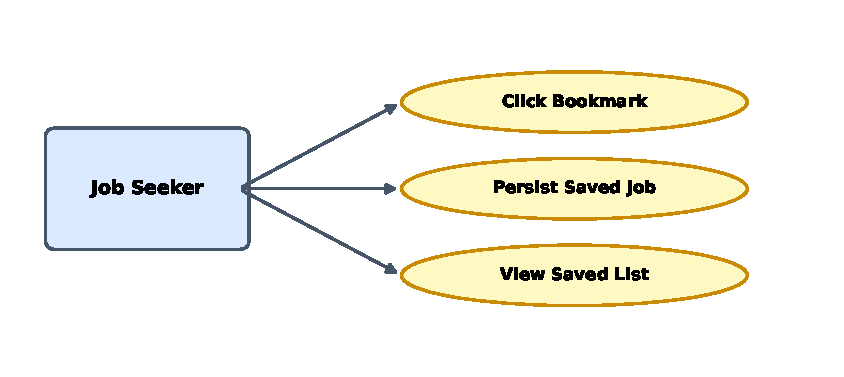
\includegraphics[width=0.65\linewidth]{figures/usecase_save_job.pdf}
\caption{Save Job to Bookmarks Use Case Diagram (UC-11)}
\label{fig:uc11_diag}
\end{figure}

\begin{table}[h!]
\centering
\small
\caption{Use Case: Save Job to Bookmarks (UC-11)}
\label{tab:uc11_spec}
\begin{tabular}{|p{3.5cm}|p{11.5cm}|}
\hline
\textbf{Use Case ID} & UC-11 \\ \hline
\textbf{Use Case Name} & Save Job to Bookmarks \\ \hline
\textbf{Created By} & RecruitSense Engineering Team \\ \hline
\textbf{Last Updated By} & Lead System Architect \\ \hline
\textbf{Actors} & Job Seeker \\ \hline
\textbf{Description} & Candidate bookmarks a job listing for future review and tracking. \\ \hline
\textbf{Trigger} & Candidate clicks the bookmark icon on any job card. \\ \hline
\textbf{Preconditions} & Candidate is logged into an active Job Seeker account. \\ \hline
\textbf{Postconditions} & Record inserted into \texttt{saved\_jobs} table; UI badge toggled. \\ \hline
\textbf{Normal Flow} & 
\textbf{Actor Actions:} \newline
1. Candidate clicks bookmark icon on a job card. \newline
\textbf{System Responses:} \newline
2. System verifies authentication. \newline
3. System inserts record into \texttt{saved\_jobs} table and updates visual bookmark state. \\ \hline
\textbf{Alternative Flows} & 1. Candidate clicks bookmark icon again to remove job from saved list. \\ \hline
\textbf{Exceptions} & 1. Unauthenticated user clicks bookmark (System prompts login modal). \\ \hline
\end{tabular}
\end{table}

\subsection{Real-Time In-App Messaging (UC-12)}
Job seekers and corporate recruiters can communicate directly within the platform regarding job inquiries, interview details, and hiring coordination. All messages are securely persisted and delivered in real time. This workflow is shown in Figure \ref{fig:uc12_diag} and specified in Table \ref{tab:uc12_spec}.

\begin{figure}[h!]
\centering
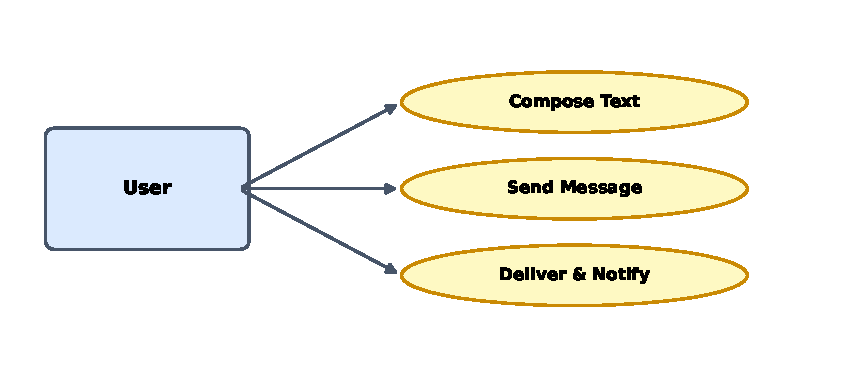
\includegraphics[width=0.65\linewidth]{figures/usecase_message.pdf}
\caption{Real-Time In-App Messaging Use Case Diagram (UC-12)}
\label{fig:uc12_diag}
\end{figure}

\begin{table}[h!]
\centering
\small
\caption{Use Case: Real-Time In-App Messaging (UC-12)}
\label{tab:uc12_spec}
\begin{tabular}{|p{3.5cm}|p{11.5cm}|}
\hline
\textbf{Use Case ID} & UC-12 \\ \hline
\textbf{Use Case Name} & Real-Time In-App Messaging \\ \hline
\textbf{Created By} & RecruitSense Engineering Team \\ \hline
\textbf{Last Updated By} & Lead System Architect \\ \hline
\textbf{Actors} & Job Seeker, Corporate Recruiter \\ \hline
\textbf{Description} & Send and receive direct messages regarding applications and interviews. \\ \hline
\textbf{Trigger} & User clicks ``Message'' on candidate profile or job application. \\ \hline
\textbf{Preconditions} & Both users are authenticated; an active application context exists. \\ \hline
\textbf{Postconditions} & Message persisted in database; recipient notified. \\ \hline
\textbf{Normal Flow} & 
\textbf{Actor Actions:} \newline
1. User selects recipient and composes message. \newline
3. User clicks ``Send''. \newline
\textbf{System Responses:} \newline
2. System sanitizes message content. \newline
4. System stores message in \texttt{messages} table, updates conversation timestamp, and alerts recipient. \\ \hline
\textbf{Alternative Flows} & 1. Recruiter attaches interview guidelines or document links. \\ \hline
\textbf{Exceptions} & 1. Message exceeds maximum character limit. \newline 2. User has been suspended. \\ \hline
\end{tabular}
\end{table}

\subsection{Schedule Candidate Interview (UC-13)}
When a candidate is moved to the \textit{Interview Scheduled} stage, the recruiter can set the interview date, time, format (In-Person or Virtual), meeting link, and candidate preparation instructions. This workflow is shown in Figure \ref{fig:uc13_diag} and specified in Table \ref{tab:uc13_spec}.

\begin{figure}[h!]
\centering
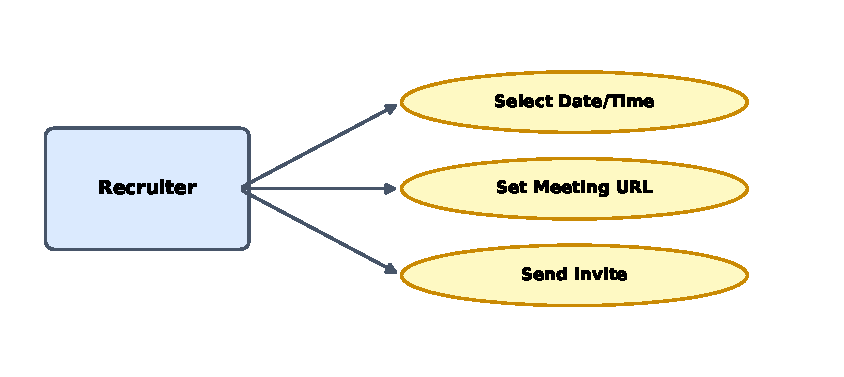
\includegraphics[width=0.65\linewidth]{figures/usecase_interview.pdf}
\caption{Schedule Candidate Interview Use Case Diagram (UC-13)}
\label{fig:uc13_diag}
\end{figure}

\begin{table}[h!]
\centering
\small
\caption{Use Case: Schedule Candidate Interview (UC-13)}
\label{tab:uc13_spec}
\begin{tabular}{|p{3.5cm}|p{11.5cm}|}
\hline
\textbf{Use Case ID} & UC-13 \\ \hline
\textbf{Use Case Name} & Schedule Candidate Interview \\ \hline
\textbf{Created By} & RecruitSense Engineering Team \\ \hline
\textbf{Last Updated By} & Lead System Architect \\ \hline
\textbf{Actors} & Corporate Recruiter / Employer \\ \hline
\textbf{Description} & Recruiter configures interview schedule, meeting location, and candidate instructions. \\ \hline
\textbf{Trigger} & Recruiter selects ``Schedule Interview'' on a shortlisted applicant card. \\ \hline
\textbf{Preconditions} & Candidate application is in \textit{Shortlisted} or \textit{Interview} status. \\ \hline
\textbf{Postconditions} & \texttt{interview\_at} and \texttt{interview\_location} saved; candidate notified. \\ \hline
\textbf{Normal Flow} & 
\textbf{Actor Actions:} \newline
1. Recruiter selects date and time. \newline
3. Recruiter specifies meeting URL (e.g., Google Meet / Teams) or physical address. \newline
5. Recruiter clicks ``Confirm Schedule''. \newline
\textbf{System Responses:} \newline
2. System validates date is in the future. \newline
4. System sanitizes location text. \newline
6. System updates application record, advances status to \textit{Interview Scheduled}, and dispatches notification. \\ \hline
\textbf{Alternative Flows} & 1. Recruiter reschedules an existing interview date. \\ \hline
\textbf{Exceptions} & 1. Past date selected (Validation error displayed). \\ \hline
\end{tabular}
\end{table}

\subsection{Verify Corporate Email Domain (UC-14)}
To prevent fraudulent employers and fake postings, the system validates recruiter email domains during registration and profile creation. Platform administrators can also manually inspect and verify employer organizations. This workflow is shown in Figure \ref{fig:uc14_diag} and specified in Table \ref{tab:uc14_spec}.

\begin{figure}[h!]
\centering
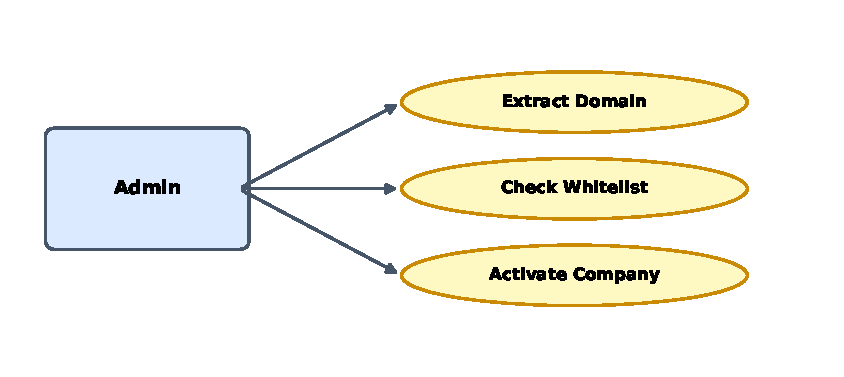
\includegraphics[width=0.65\linewidth]{figures/usecase_domain_verify.pdf}
\caption{Verify Corporate Email Domain Use Case Diagram (UC-14)}
\label{fig:uc14_diag}
\end{figure}

\begin{table}[h!]
\centering
\small
\caption{Use Case: Verify Corporate Email Domain (UC-14)}
\label{tab:uc14_spec}
\begin{tabular}{|p{3.5cm}|p{11.5cm}|}
\hline
\textbf{Use Case ID} & UC-14 \\ \hline
\textbf{Use Case Name} & Verify Corporate Email Domain \\ \hline
\textbf{Created By} & RecruitSense Engineering Team \\ \hline
\textbf{Last Updated By} & Lead System Architect \\ \hline
\textbf{Actors} & Administrator, Validation Engine \\ \hline
\textbf{Description} & Verify legitimacy of corporate employer email domains and activate posting privileges. \\ \hline
\textbf{Trigger} & Recruiter registers or administrator reviews company pending queue. \\ \hline
\textbf{Preconditions} & Recruiter has submitted company registration details. \\ \hline
\textbf{Postconditions} & \texttt{companies.verified} flag set to \texttt{true}; verified badge displayed. \\ \hline
\textbf{Normal Flow} & 
\textbf{System / Admin Actions:} \newline
1. System extracts domain from recruiter email (e.g., \texttt{@techcorp.com}). \newline
2. Validation rule checks against disposable domain blacklists. \newline
3. Administrator reviews corporate website and tax/registration details if required. \newline
4. System sets \texttt{verified = true} and unlocks job publishing capabilities. \\ \hline
\textbf{Alternative Flows} & 1. Admin rejects fraudulent company profile with explanation. \\ \hline
\textbf{Exceptions} & 1. Recruiter registered with generic disposable email (System flags profile). \\ \hline
\end{tabular}
\end{table}

\subsection{Moderate Employer Accounts (UC-15)}
Administrators review pending or reported employer accounts to ensure compliance with recruitment guidelines and fair hiring practices. This workflow is shown in Figure \ref{fig:uc15_diag} and specified in Table \ref{tab:uc15_spec}.

\begin{figure}[h!]
\centering
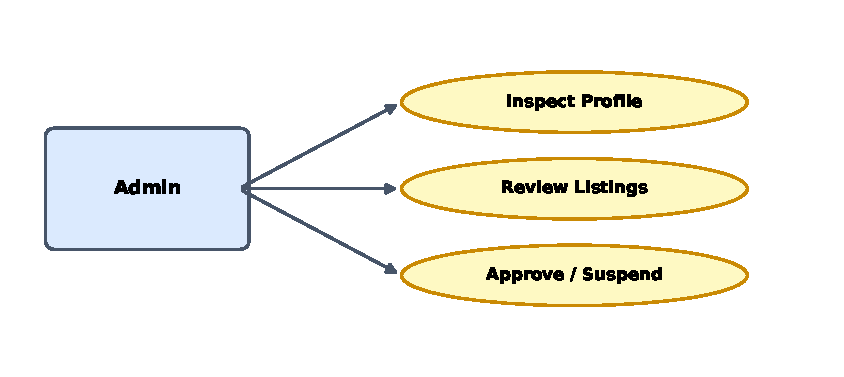
\includegraphics[width=0.65\linewidth]{figures/usecase_moderate_employer.pdf}
\caption{Moderate Employer Accounts Use Case Diagram (UC-15)}
\label{fig:uc15_diag}
\end{figure}

\begin{table}[h!]
\centering
\small
\caption{Use Case: Moderate Employer Accounts (UC-15)}
\label{tab:uc15_spec}
\begin{tabular}{|p{3.5cm}|p{11.5cm}|}
\hline
\textbf{Use Case ID} & UC-15 \\ \hline
\textbf{Use Case Name} & Moderate Employer Accounts \\ \hline
\textbf{Created By} & RecruitSense Engineering Team \\ \hline
\textbf{Last Updated By} & Lead System Architect \\ \hline
\textbf{Actors} & Platform Administrator \\ \hline
\textbf{Description} & Administrator audits and moderates corporate employer accounts and job listings. \\ \hline
\textbf{Trigger} & Administrator opens the Admin Company Moderation dashboard. \\ \hline
\textbf{Preconditions} & Administrator is authenticated with \texttt{'admin'} role. \\ \hline
\textbf{Postconditions} & Employer account status updated (Approved, Flagged, Suspended). \\ \hline
\textbf{Normal Flow} & 
\textbf{Actor Actions:} \newline
1. Admin accesses employer queue. \newline
3. Admin inspects company profile, active vacancies, and reported flags. \newline
5. Admin approves or suspends company posting privileges. \newline
\textbf{System Responses:} \newline
2. System loads company records with verification statuses. \newline
4. System displays company metrics. \newline
6. System updates status, deactivates listings if suspended, and logs audit trail. \\ \hline
\textbf{Alternative Flows} & 1. Admin sends informational warning to company. \\ \hline
\textbf{Exceptions} & 1. Insufficient administrative privileges (HTTP 403 error). \\ \hline
\end{tabular}
\end{table}

\subsection{Moderate User Accounts and Suspensions (UC-16)}
Platform administrators can manage user accounts, investigate policy violations, issue formal warnings, and suspend abusive users (e.g., spam job seekers or fraudulent recruiters). This workflow is shown in Figure \ref{fig:uc16_diag} and specified in Table \ref{tab:uc16_spec}.

\begin{figure}[h!]
\centering
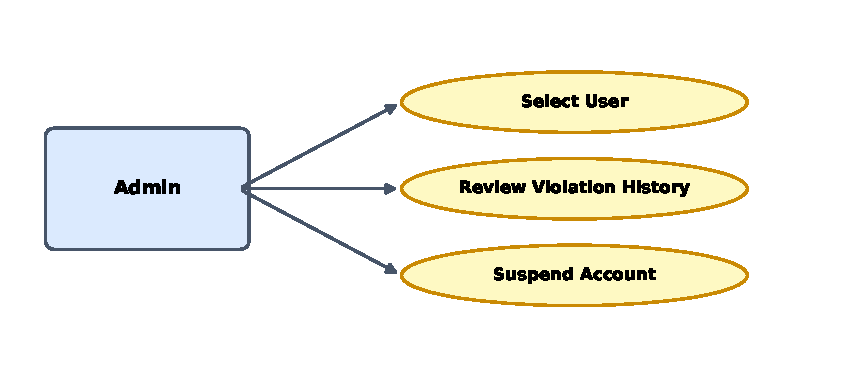
\includegraphics[width=0.65\linewidth]{figures/usecase_moderate_users.pdf}
\caption{Moderate User Accounts Use Case Diagram (UC-16)}
\label{fig:uc16_diag}
\end{figure}

\begin{table}[h!]
\centering
\small
\caption{Use Case: Moderate User Accounts and Suspensions (UC-16)}
\label{tab:uc16_spec}
\begin{tabular}{|p{3.5cm}|p{11.5cm}|}
\hline
\textbf{Use Case ID} & UC-16 \\ \hline
\textbf{Use Case Name} & Moderate User Accounts and Suspensions \\ \hline
\textbf{Created By} & RecruitSense Engineering Team \\ \hline
\textbf{Last Updated By} & Lead System Architect \\ \hline
\textbf{Actors} & Platform Administrator \\ \hline
\textbf{Description} & Admin reviews reported user behavior and applies suspensions or restrictions. \\ \hline
\textbf{Trigger} & Admin accesses user moderation panel. \\ \hline
\textbf{Preconditions} & Admin is authenticated; reported user exists. \\ \hline
\textbf{Postconditions} & User status changed to \texttt{'suspended'}; active sessions terminated. \\ \hline
\textbf{Normal Flow} & 
\textbf{Actor Actions:} \newline
1. Admin selects flagged user account. \newline
3. Admin reviews violation logs and submitted reports. \newline
5. Admin confirms suspension and enters reason. \newline
\textbf{System Responses:} \newline
2. System loads profile history and activity. \newline
4. System displays action options. \newline
6. System sets \texttt{users.status = 'suspended'}, revokes Sanctum tokens, and sends email notice. \\ \hline
\textbf{Alternative Flows} & 1. Admin lifts previous suspension after appeal review. \\ \hline
\textbf{Exceptions} & 1. Admin attempts to suspend own account (Action blocked). \\ \hline
\end{tabular}
\end{table}

\subsection{View System Analytics and Audit Logs (UC-17)}
Administrators can inspect global recruitment analytics, including total registered candidates, verified employers, active job listings, total resumes parsed, average ATS match scores across categories, and system API logs. This workflow is shown in Figure \ref{fig:uc17_diag} and specified in Table \ref{tab:uc17_spec}.

\begin{figure}[h!]
\centering
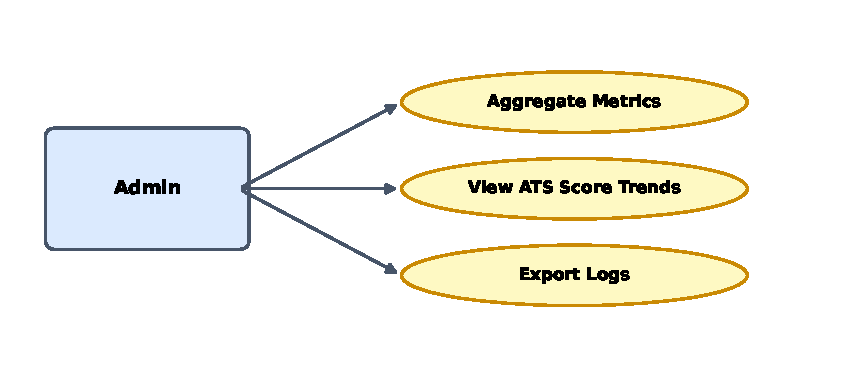
\includegraphics[width=0.65\linewidth]{figures/usecase_analytics.pdf}
\caption{View System Analytics Use Case Diagram (UC-17)}
\label{fig:uc17_diag}
\end{figure}

\begin{table}[h!]
\centering
\small
\caption{Use Case: View System Analytics and Audit Logs (UC-17)}
\label{tab:uc17_spec}
\begin{tabular}{|p{3.5cm}|p{11.5cm}|}
\hline
\textbf{Use Case ID} & UC-17 \\ \hline
\textbf{Use Case Name} & View System Analytics and Audit Logs \\ \hline
\textbf{Created By} & RecruitSense Engineering Team \\ \hline
\textbf{Last Updated By} & Lead System Architect \\ \hline
\textbf{Actors} & Platform Administrator \\ \hline
\textbf{Description} & Administrator monitors global platform statistics, ATS screening metrics, and activity logs. \\ \hline
\textbf{Trigger} & Admin opens Admin Analytics Dashboard. \\ \hline
\textbf{Preconditions} & Admin is authenticated with root permissions. \\ \hline
\textbf{Postconditions} & Statistical visual metrics and system audit logs rendered. \\ \hline
\textbf{Normal Flow} & 
\textbf{Actor Actions:} \newline
1. Admin navigates to Analytics tab. \newline
3. Admin selects date range filter. \newline
\textbf{System Responses:} \newline
2. System aggregates database metrics (users, jobs, applications, average ATS scores). \newline
4. System updates graphical charts and performance summaries in real time. \\ \hline
\textbf{Alternative Flows} & 1. Admin exports platform health metrics to CSV/JSON report. \\ \hline
\textbf{Exceptions} & 1. Database query timeout during high-volume aggregation. \\ \hline
\end{tabular}
\end{table}

\subsection{Update Profile and Professional Summary (UC-18)}
Job seekers and recruiters can update their personal profiles, headline, biography, portfolio links, location, and technical skill tags. This workflow is shown in Figure \ref{fig:uc18_diag} and specified in Table \ref{tab:uc18_spec}.

\begin{figure}[h!]
\centering
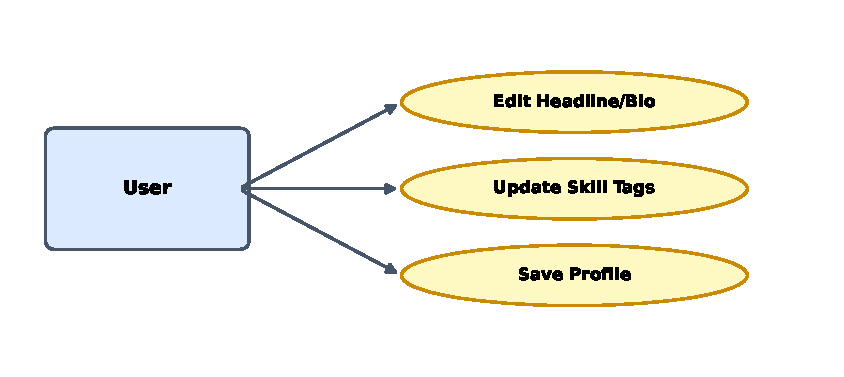
\includegraphics[width=0.65\linewidth]{figures/usecase_profile.pdf}
\caption{Update Profile Use Case Diagram (UC-18)}
\label{fig:uc18_diag}
\end{figure}

\begin{table}[h!]
\centering
\small
\caption{Use Case: Update Profile and Professional Summary (UC-18)}
\label{tab:uc18_spec}
\begin{tabular}{|p{3.5cm}|p{11.5cm}|}
\hline
\textbf{Use Case ID} & UC-18 \\ \hline
\textbf{Use Case Name} & Update Profile and Professional Summary \\ \hline
\textbf{Created By} & RecruitSense Engineering Team \\ \hline
\textbf{Last Updated By} & Lead System Architect \\ \hline
\textbf{Actors} & Registered User (Job Seeker, Recruiter) \\ \hline
\textbf{Description} & Modify personal details, bio, skill tags, contact details, and account preferences. \\ \hline
\textbf{Trigger} & User clicks ``Edit Profile'' on their profile dashboard. \\ \hline
\textbf{Preconditions} & User is authenticated. \\ \hline
\textbf{Postconditions} & Profile record updated in database; updated data reflected in client state. \\ \hline
\textbf{Normal Flow} & 
\textbf{Actor Actions:} \newline
1. User accesses profile settings. \newline
3. User edits bio, location, headline, or adds new skills. \newline
5. User clicks ``Save Profile''. \newline
\textbf{System Responses:} \newline
2. System loads current profile data. \newline
4. System validates character lengths and inputs. \newline
6. System updates \texttt{job\_seekers} or \texttt{companies} table and displays success alert. \\ \hline
\textbf{Alternative Flows} & 1. User toggles Dark/Light theme mode in profile settings. \\ \hline
\textbf{Exceptions} & 1. Invalid input format (System highlights erroneous fields). \\ \hline
\end{tabular}
\end{table}

\subsection{Report Suspicious or Fraudulent Job Posting (UC-19)}
Job seekers can report misleading, discriminatory, or fraudulent job listings directly through the job details interface. The report includes category selection (e.g., Fake Listing, Scam, Inappropriate Content) and supporting remarks, adding the case to the admin moderation queue. This workflow is shown in Figure \ref{fig:uc19_diag} and specified in Table \ref{tab:uc19_spec}.

\begin{figure}[h!]
\centering
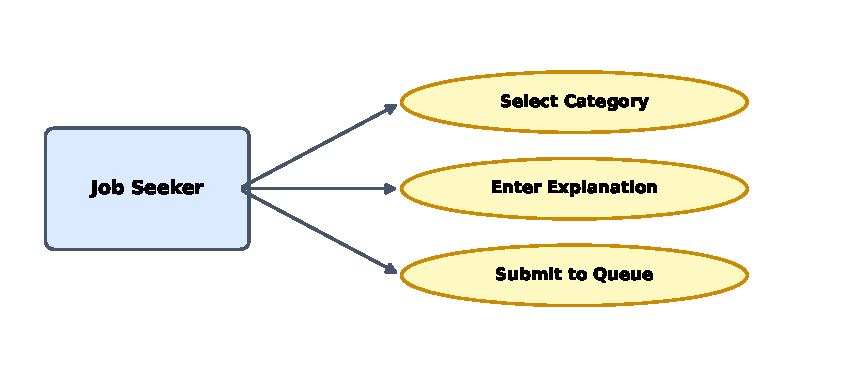
\includegraphics[width=0.65\linewidth]{figures/usecase_report_job.pdf}
\caption{Report Fraudulent Job Posting Use Case Diagram (UC-19)}
\label{fig:uc19_diag}
\end{figure}

\begin{table}[h!]
\centering
\small
\caption{Use Case: Report Suspicious or Fraudulent Job Posting (UC-19)}
\label{tab:uc19_spec}
\begin{tabular}{|p{3.5cm}|p{11.5cm}|}
\hline
\textbf{Use Case ID} & UC-19 \\ \hline
\textbf{Use Case Name} & Report Suspicious or Fraudulent Job Posting \\ \hline
\textbf{Created By} & RecruitSense Engineering Team \\ \hline
\textbf{Last Updated By} & Lead System Architect \\ \hline
\textbf{Actors} & Job Seeker \\ \hline
\textbf{Description} & Candidate flags a job posting for policy violations or fraudulent behavior. \\ \hline
\textbf{Trigger} & Candidate clicks ``Report Job'' on a job vacancy modal. \\ \hline
\textbf{Preconditions} & Candidate is authenticated; job posting is active. \\ \hline
\textbf{Postconditions} & Report record inserted into database; listing flagged for admin review. \\ \hline
\textbf{Normal Flow} & 
\textbf{Actor Actions:} \newline
1. Candidate clicks ``Report Job''. \newline
3. Candidate selects violation category and inputs explanation. \newline
5. Candidate clicks ``Submit Report''. \newline
\textbf{System Responses:} \newline
2. System displays report modal. \newline
4. System validates completeness of explanation. \newline
6. System persists report, notifies admin queue, and confirms submission to user. \\ \hline
\textbf{Alternative Flows} & 1. Candidate cancels report modal before submitting. \\ \hline
\textbf{Exceptions} & 1. Candidate has already submitted a report for this job. \\ \hline
\end{tabular}
\end{table}

\subsection{Review Reported Content and Job Postings (UC-20)}
Administrators review reported job postings and candidate complaints, examine evidence, and take administrative action—such as removing the listing, warning the employer, or dismissing false reports. This workflow is shown in Figure \ref{fig:uc20_diag} and specified in Table \ref{tab:uc20_spec}.

\begin{figure}[h!]
\centering
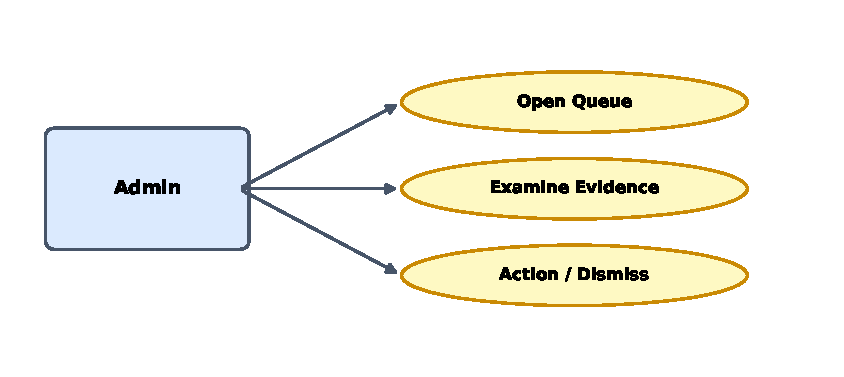
\includegraphics[width=0.65\linewidth]{figures/usecase_review_reports.pdf}
\caption{Review Reported Content Use Case Diagram (UC-20)}
\label{fig:uc20_diag}
\end{figure}

\begin{table}[h!]
\centering
\small
\caption{Use Case: Review Reported Content and Job Postings (UC-20)}
\label{tab:uc20_spec}
\begin{tabular}{|p{3.5cm}|p{11.5cm}|}
\hline
\textbf{Use Case ID} & UC-20 \\ \hline
\textbf{Use Case Name} & Review Reported Content and Job Postings \\ \hline
\textbf{Created By} & RecruitSense Engineering Team \\ \hline
\textbf{Last Updated By} & Lead System Architect \\ \hline
\textbf{Actors} & Platform Administrator \\ \hline
\textbf{Description} & Administrator mediates complaints, reviews flagged content, and applies policy enforcement. \\ \hline
\textbf{Trigger} & Administrator accesses the Admin Reports Queue. \\ \hline
\textbf{Preconditions} & Administrator is authenticated with moderation privileges. \\ \hline
\textbf{Postconditions} & Reported issue is resolved; listing removed or report dismissed. \\ \hline
\textbf{Normal Flow} & 
\textbf{Actor Actions:} \newline
1. Admin opens reported content queue. \newline
3. Admin selects report to inspect. \newline
5. Admin decides outcome (Remove Listing, Suspend Employer, or Dismiss). \newline
\textbf{System Responses:} \newline
2. System displays list of unresolved reports. \newline
4. System presents job details, employer history, and reporter comments. \newline
6. System executes decision, updates database, and notifies reporting user. \\ \hline
\textbf{Alternative Flows} & 1. Admin sends warning message to employer requesting listing revision. \\ \hline
\textbf{Exceptions} & 1. Job posting was already deleted by owner prior to review. \\ \hline
\end{tabular}
\end{table}

\section{Chapter Summary}
This chapter comprehensively documented the requirement specifications for \textbf{RecruitSense}. It analyzed the operational bottlenecks of existing manual and keyword-based recruitment systems, articulated the proposed platform capabilities, established the functional requirements (FR-01 to FR-20) and non-functional quality constraints (NFR-01 to NFR-10), presented the overall system use case model, and provided formal tabular specifications alongside native vector diagrams for 20 distinct use cases. These specifications establish a rigorous foundation for the architectural and system design detailed in Chapter \ref{chap:design}.
